% -*-coding: utf-8-*-
% This is an AMS-LaTeX v. 1.2 File.

\documentclass{report}

%\usepackage{pscyr}
%\renewcommand{\rmdefault}{fjn}
%\renewcommand{\ttdefault}{fcr}

%\usepackage{showkeys}
\usepackage[T2A]{fontenc}
\usepackage[utf8x]{inputenc}
\usepackage[english,russian]{babel}
\usepackage{expdlist}
\usepackage[pdftex]{graphicx}
\usepackage{amsmath}
\usepackage{amssymb}
\usepackage{amsthm}
\usepackage{amsfonts}
\usepackage{amsxtra} 
\usepackage{sty/dbl12}
\usepackage{srcltx}
\usepackage{epsfig}
\usepackage{verbatim}
\usepackage{cite}
\usepackage{sty/rac}
%\usepackage[russian]{sty/ralg}
\usepackage{listings}
\usepackage{placeins}
%\usepackage{floatrow}
\usepackage{caption}
\captionsetup[table]{position=t}
\usepackage{multirow}
\usepackage{arydshln}
\usepackage{url}
\mathchardef\UrlBreakPenalty=10000
\mathchardef\UrlBigBreakPenalty=10000

%\usepackage[
%    top    = 2.00cm,
%    bottom = 2.00cm,
%    left   = 3.00cm,
%    right  = 1.50cm]{geometry}
\hoffset = -10mm
\voffset = -20mm
\textheight = 230mm
\textwidth = 165mm

\begin{document}

% Begin the front matter as required by Rackham dissertation guidelines

\initializefrontsections

\pagestyle{title}

\begin{center}
Санкт-Петербургский национальный исследовательский университет \\ информационных технологий, механики и оптики

\vspace{2cm}

Факультет информационных технологий и программирования

Кафедра компьютерных технологий

\vspace{3cm}

{\Large Мельник Михаил Валерьевич}

\vspace{2cm}

\vbox{\LARGE\bfseries
Применение методов решения задачи о выполнимости булевой формулы для построения минимальной филогенетической сети}

\vspace{4cm}

{\Large Научный руководитель: аспирант кафедры КТ В.~И.~Ульянцев}

\vspace{6cm}

Санкт-Петербург\\ 2015
\end{center}

\newpage

\setcounter{page}{3}
\pagestyle{plain}

%\dedicationpage{Put a dedication here}
% Dedication page

%\startacknowledgementspage
% Acknowledgements page
%{Put Acknowledgements here}

% Table of contents, list of figures, etc.
\tableofcontents
%\listoffigures

% Chapters
\startthechapters
% -*-coding: utf-8-*-
\startprefacepage

Построение минимальной филогенетической сети является важной задачей филогенетики.
Филогенетическая сеть используется для представления эволюционных взаимосвязей между различными биологическими видами в ретикулярной модели эволюции.
В ретикулярной (сетчатой) модели эволюции, в отличие от классической (древовидной) модели, присутствует горизонтальный перенос генов, а также гибридизация между видами, что не позволяет использовать более простые структуры, такие как филогенетические деревья.
Филогенетические сети активно исследуются в настоящее время~\cite{huson2010phylogenetic, morrison2011introduction, 
nakhleh2011evolutionary}.

Хотя существует несколько формальных определений филогенетических сетей, в данной работе рассматриваются только гибридизационные сети~\cite{semple2006hybridization, chen2010hybridnet}.
Исходными данными для построения гибридизационной сети является набор из нескольких филогенетических деревьев, построенных на одном и том же множестве таксонов.
Каждое филогенетическое дерево представляет собой эволюционную историю какого-то гена.
Деревья могут иметь различную топологию из-за наличия ретикуляций.
Задача состоит в том, чтобы построить гибридизационную сеть с минимальным количеством вершин, содержащую в себе каждое из исходных деревьев как подграф.

Большинство алгоритмов для построения гибридизационных сетей основаны на эвристиках и не гарантируют точный результат~\cite{wu2010close, park2012murpar}.
Кроме того, многие алгоритмы не могут работать более чем с двумя деревьями.
Недавно был представлен точный алгоритм, работающий с многими деревьями~\cite{wu2013algorithm}.
С точной и эвристической версией этого алгоритма, как с наиболее производительной на текущий момент, будет производиться сравнение.

В данной работе представлен новый способ построения минимальной гибридизационной сети, основанный на сведении к задаче о выполнимости булевой формулы (SAT), гарантирующий точный результат.
На основе представленного алгоритма была разработана утилита PhyloSAT, решающая поставленную задачу. Исходный код утилиты доступен на GitHub\footnote{\url{https://github.com/ctlab/PhyloSAT}}.

Подходы, основывающиеся на сведении к задаче SAT, успешно применяются для решения различных задач, в том числе для задач филогенетики~\cite{bonet2009efficiently}, построения конечных автоматов~\cite{heule2010exact} и верификации~\cite{biere2003bounded}.
Это обусловлено тем, что современные SAT-солверы хорошо оптимизированы, и способны успешно справляться с формулами из десятков тысяч переменных за несколько минут.

%-*-coding: utf-8-*-
\FloatBarrier
\chapter{Обзор предметной области}

\FloatBarrier
\section{Основные определения}

\subsection{Филогенетика}

\emph{Филогенетика} --- область биологической систематики, которая занимается идентификацией и прояснением эволюционных взаимоотношений среди разных видов жизни на Земле~\cite{wiki:phylogenetics}.

\emph{Филогенетическим деревом} называется дерево, отражающее эволюционные взаимосвязи между различными видами или другими сущностями, имеющими общего предка~\cite{wiki:phylogenetic-tree}.
В данной работе будут рассматриваться подвешенные двоичные деревья. Листья филогенетического дерева отображают таксоны, а узлы представляют из себя эволюционные события: разделение предкового вида на два независимых.
Примеры филогенетических деревьев показаны на Рис.~\ref{input-example}.

\emph{Гибридизационная сеть} --- направленный ациклический граф с выделенным корнем.
Гибридизационная сеть состоит из трех типов вершин - обычных вершин, ретикулярных вершин и листьев.
Обычные вершины имеют одного предка и нескольких потомков.
\emph{Ретикулярные вершины} имеют более одного предка и нескольких потомков.
Листья имеют одного предка и не имеют потомков.
В данной работе, без потери общности, будет рассматриваться упрощенная модель гибридизационной сети, в которой обычные вершины имеют ровно двух потомков, а ретикулярные вершины имеют ровно двух предков и ровно одного потомка. 
Заметим, что привести произвольную гибридизационную сеть к упрощенному виду не составляет труда~\cite{wu2010close}.
Примеры гибридизационных сетей показаны на Рис.~\ref{network-example}.

\begin{figure}[t]
  \centering
  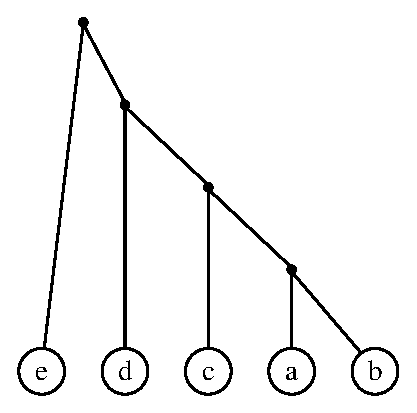
\includegraphics[width=4cm]{img/inp1.eps}
  \hspace{5mm}
  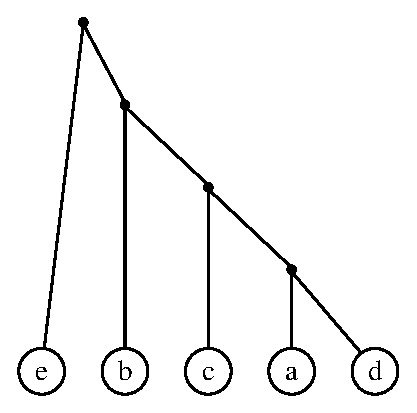
\includegraphics[width=4cm]{img/inp2.eps}
  \hspace{5mm}
  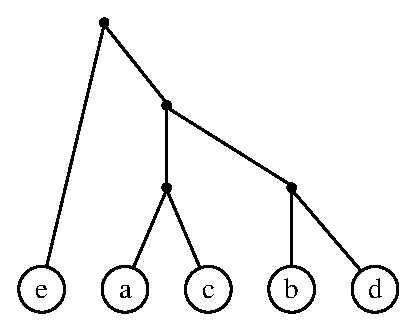
\includegraphics[width=4cm]{img/inp3.eps}
  \caption{Три филогенетических дерева над множеством таксонов \{a, b, c, d, e\}.}
  \label{input-example}
\end{figure}

\begin{figure}[t]
  \centering
  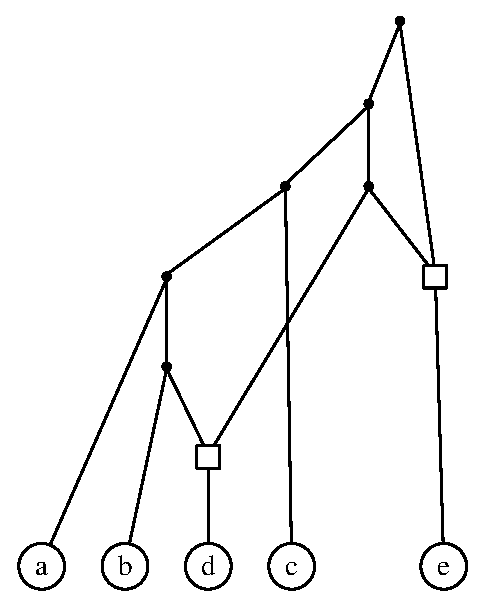
\includegraphics[width=4cm]{img/ans.eps}
  \hspace{1cm}
  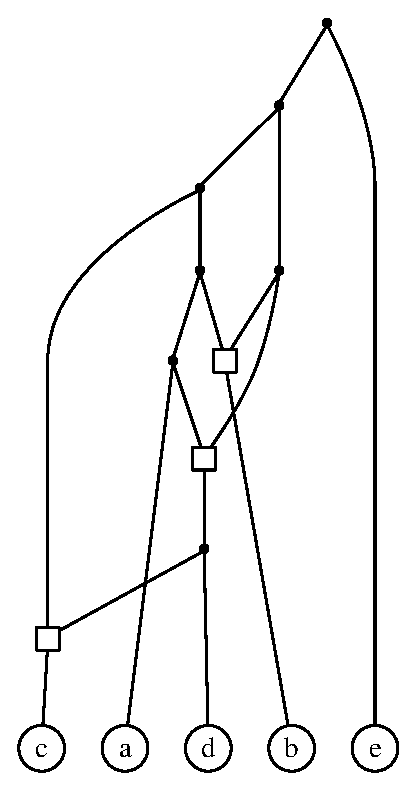
\includegraphics[width=4cm]{img/ans3.eps}
  \caption{Возможные гибридизационные сети, для деревьев из Рис.~\ref{input-example}, с двумя и тремя ретикулярными событиями соответственно. Ретикулярные вершины обозначены квадратиками.}
  \label{network-example}
\end{figure}

Гибридизационную сеть можно свести к филогенетическому дереву следующим образом:

\begin{itemize}
	\item У каждой ретикулярной вершины необходимо выбрать используемого предка, а ребро ведущее к другому предку удалить.
	\item Если у ретикулярной вершины удалено ребро, ведущее в её единственного сына, то ретикулярную вершину также следует удалить.
	\item Стянуть все ребра, имеющие ровно одного предка и ровно одного потомка.
\end{itemize}

Гибридизационная сеть $N$ \emph{отображает} дерево $T$, если существует такой способ выбора удаляемых ребер, что после стягивания получится дерево $T'$ изоморфное дереву $T$.
При этом, вершины сети, которые остались после стягивания ребер, будем называть вершинами \emph{используемыми для отображения} дерева $t$.
Гибридизационные сети на Рис.~\ref{network-example} содержат в себе все три дерева из Рис.~\ref{input-example}.

\emph{Гибридизационным числом} сети $N$ с корнем $\rho$ называется величина $h(N) = \sum\limits_{v \ne \rho} (d^-(v) - 1)$, где за $d^-(v)$ обозначена входящая степень вершины $v$.
Аналогично обозначим за $d^+(v)$ исходящую степень вершины $v$.
Заметим, что в нашей модели значение $h(N)$ равно количеству ретикулярных вершин.

Рассмотрим множество из $k$ филогенетических деревьев $T_1, T_2, \dots, T_k$, построенных над фиксированным множеством таксонов.
Сеть $N_{min}$ называется \emph{минимальной гибридизационной сетью}, если она принадлежит множеству сетей, содержащих в себе все $k$ деревьев, и при этом имеет наименьшее возможное гибридизационное число.

Множество таксонов $A$ называется \emph{кластером} на деревьях $T_1, T_2, \dots, T_k$, если в каждом дереве $T_i$ существует вершина $v_i$, такая, что множество листьев в поддереве $v_i$ совпадает с множеством $A$.

\subsection{Выполнимость булевой формулы}

\emph{Задача о выполнимости булевой формулы (SAT)} заключается в следующем: можно ли назначить всем переменным, встречающимся в формуле, значения ложь и истина так, чтобы формула стала истинной~\cite{wiki:sat}. Обычно рассматриваются формулы в конъюктивной нормальной форме.

\emph{SAT-солвер} --- программа предназначенная для решения задачи выполнимости булевой формулы.

\FloatBarrier
\section{Постановка задачи}

Задача построения минимальной гибридизационной сети заключается в том, чтобы для множества филогенетических деревьев $T_1, T_2, \dots, T_k$ построить минимальную гибридизационную сеть.

Было показано, что даже для случая двух деревьев эта задача NP-полна~\cite {bordewich2007computing}.

\FloatBarrier
\section{Обзор существующих методов}

%-*-coding: utf-8-*-
\FloatBarrier
\chapter{Описание используемого подхода}

\FloatBarrier
\section{Основная идея}

Идея заключается в составлении булевой формулы для набора входных деревьев и гибридизационного числа $h$, которая выполнима тогда и только тогда, когда существует гибридизационная сеть $N_h$ с гибридизационным числом $h$, содержащая в себе все входные деревья.
Определив диапазон возможных значений гибридизационного числа, можно перебрать их все и составить формулы для фиксированных значений гибридизационного числа.
В итоге, ответом на задачу будет та из выполнимых формул, которая соответствует наименьшему гибридизационному числу.

\FloatBarrier
\section{Препроцессинг}

Перед тем как приступать к непосредственному кодированию булевой формулы, применяются несколько эвристик, позволяющих разбить задачу на подзадачи, и следовательно уменьшить её сложность.
Для разбиения применяются следующие правила~\cite{bonet2009efficiently}:

\begin{enumerate}
	\item \textbf{Сокращение поддерева.} Если существует поддерево, содержащееся в каждом из исходных деревьев, значит в этой части эволюционной истории не наблюдалось ретикуляций, и для её отображения достаточно древовидной структуры.
	Поэтому во всех исходных деревьях следует заменить это поддерево на лист с новой меткой.
	После решения задачи, в готовой сети, следует заменить этот лист на исходное поддерево.
	\item \textbf{Сокращение кластера.} Если существует кластер $A$, содержащийся в каждом из исходных деревьев, его также следует заменить на лист с новой меткой, а задачу построения минимальной гибридизационной сети решать для этого кластера отдельно.
	После решения задачи, следует заменить этот лист в готовой сети на сеть, являющуюся решением задачи для кластера $A$.
\end{enumerate}

Предложенный далее алгоритм предполагает, что у всех входных деревьев общий корень, но это предположение не выполняется для построенных подзадач.
Поэтому следует добавить фиктивный корень ко всем деревьям в каждой из подзадач.
Чтобы сохранить структуру деревьев корень добавляется вместе с новым фиктивным листом.
Этот процесс проиллюстрирован на Рис.~\ref{dummy-example}.
После решения задачи, фиктивный корень и фиктивный лист следует удалить.

\begin{figure}[t]
  \centering{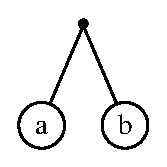
\includegraphics[width=2.6cm]{img/inp_dummy.eps}}
  \hspace{2cm}
  \centering{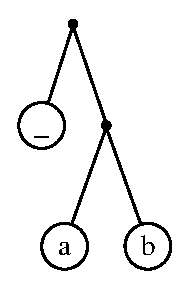
\includegraphics[width=3cm]{img/ans_dummy.eps}}
  \caption{Добавление фиктивного корня к дереву.}
  \label{dummy-example}
\end{figure}

\FloatBarrier
\section{Перебор гибридизационного числа}

Для решения задачи требуется найти такое минимальное $h$, что будет существовать гибридизационная сеть с гибридизационным числом равным $h$.
Существует несколько методик перебора значения $h$: последовательный перебор от больших значений к маленьким, от маленьких значений к большим и двоичный поиск.
В рамках данной работы были реализованы все три методики.
Если минимальное гибридизационное число равно $h_\mathrm{min}$, то, как правило, наибольшее количество вычислений потребуется для решения формулы при $h = h_\mathrm{min} - 1$.
Это обусловлено тем фактом, что найти какое-нибудь решение для солвера проще, чем, перебрав все варианты, убедиться, что решения не существует.
Экспериментальные результаты подтверждают это наблюдение, и поэтому перебор от маленьких значений к большим не представляет интереса, так как его производительность значительно ниже чем у остальных методов.
Результаты двоичного поиска практически повторяют результаты перебора от больших значений к маленьким, кроме случаев, в которых выполняется значительное количество проверок для значений меньших чем $h_\mathrm{min}$.


В данной работе используется перебор от больших значений к маленьким, как наиболее производительный метод.
Кроме того, было экспериментально обнаружено, что у многих из получаемых подзадач гибридизационное число мало, и времени на решение таких подзадач тратится мало, поэтому используется следующая эвристика: перед началом перебора производится попытка быстрого решения со значениями $h$ равными $0$, $1$, $2$ и $3$. В каждом из случаев солверу выделяется одна секунда на решение.


Объем вычислений можно очевидным образом сократить, если подобрать более точные границы возможных значений гибридизационного числа.
Существует несколько быстрых методов, основанных на различных эвристиках и методах линейного программирования, например PIRN$\mathrm{_{CH}}$~\cite{wu2010close}, RIATA-HGT~\cite{nakhleh2005riata} и MURPAR~\cite{park2012murpar}.

\FloatBarrier
\section{Кодирование булевой формулы}

\subsection{Общие замечания}

Обозначим исходное множество деревьев за $T$, множество таксонов за $A$, размер $A$ за $n$, а предполагаемое гибридизационное число за $h$. Требуется построить булеву формулу, которая выполнима тогда и только тогда, когда существует сеть, с гибридизационным номером $h$, в которой содержатся все деревья из $T$.

Для начала, заметим, что исходные деревья содержат $2 n - 1$ вершин, а искомая сеть состоит из $2 (n + k) + 1$ вершин, т.к. добавляется фиктивный корень и фиктивный лист. Среди этих вершин $n + 1$ лист, $k$ ретикулярных вершин, и $n + k$ обычных вершин.

Введем нумерацию вершин по следующим правилам:

\begin{enumerate}
	\item Листья будут иметь номера в диапазоне $[0, n]$.
	\item Обычные вершины будут иметь номера в диапазоне $[n + 1, 2n + k]$.
	\item Ретикулярные вершины будут иметь номера в диапазоне $[2n + k + 1, 2(n + k)]$.
	\item Номер любого листа или обычной вершины меньше номера её предка.
	\item У обычной вершины номер левого сына меньше номера правого сына.
	\item У ретикулярной вершины номер левого предка меньше номера правого предка.
\end{enumerate}

Кроме того, для каждой вершины $v$, введем следующие обозначения:

\begin{itemize}
	\item $\mathrm{PC}(v)$ --- множество возможных детей вершины $v$
	\item $\mathrm{PP}(v)$ --- множество возможных предков вершины $v$
	\item $\mathrm{PU}(v)$ --- множество вершин, которые могут находиться выше вершины $v$ в сети
\end{itemize}

А также обозначим множество листьев за $L$, множество ретикулярных вершин за $R$, а множество обычных вершин за $V$.

\subsection{Кодирование структуры сети}

Чтобы закодировать структуру сети потребуются следующие переменные:

\begin{itemize}
	\item $l_{v,u}$ и $r_{v,u}$, где $v \in V, u \in PC(v)$. \\
	$l_{v,u}$ ($r_{v,u}$) истинно тогда и только тогда, когда вершина $u$ является левым (правым) ребенком вершины $v$.
	\item $p_{v,u}$, где $v \in L \cup V \backslash \{\rho\}, u \in PP(v)$. \\
	$p_{v,u}$ истинно тогда и только тогда, когда вершина $u$ является предком вершины $v$.
	\item $p^l_{v,u}$ и $p^r_{v,u}$, где $v \in R, u \in PP(v)$. \\
	$p^l_{v,u}$ ($p^r_{v,u}$) истинно тогда и только тогда, когда вершина $u$ является левым (правым) предком ретикулярной вершины $v$.
	\item $c_{v,u}$, где $v \in R, u \in PC(v)$. \\
	$c_{v,u}$ истинно тогда и только тогда, когда вершина $u$ является ребенком ретикулярной вершины $v$.
\end{itemize}

Всего требуется $O((n + k)^2)$ переменных.


\subsection{Кодирование связей исходных деревьев с сетью}

\FloatBarrier
\section{Решение булевой формулы и постпроцессинг}

Выбор подходящего солвера является темой для отдельного исследования. Некоторые эксперименты уже проводились~\cite{bonet2009efficiently}, и результаты отдельных солверов значительно превосходят результаты других. Не смотря на это, в рамках данной работы такие эксперименты не проводились. Для решения булевой формулы используется солвер CryptoMiniSat 4.2.0~\cite{cryptominisat}.

После того, как решена формула соответствующая минимальной гибридизационной сети, по полученным значениям переменных восстанавливается структура сети, удаляются фиктивный корень и фиктивный лист.
Затем, сети, полученные в результате решения подзадач, объединяются в одну сеть, являющуюся решением исходной задачи.
%-*-coding: utf-8-*-
\FloatBarrier
\chapter{Тестирование и результаты}

\FloatBarrier
\section{Описание эксперимента}

\FloatBarrier
\startconclusionpage

В данной работе предложен алгоритм построения минимальной гибридизационной сети из нескольких филогенетических деревьев, гарантирующий точный результат.
Предложенный алгоритм был реализован в программе PhyloSAT, исходный код которой доступен на GitHub\footnote{\url{https://github.com/ctlab/PhyloSAT}}.
Представленный алгоритм превосходит точный алгоритм $\mathrm{PIRN_C}$ во всех проведенных экспериментах и даже составляет конкуренцию эвристическому алгоритму $\mathrm{PIRN_{CH}}$, который не гарантирует точный результат.

В работе были рассмотрены возможные способы улучшения предложенного алгоритма, которые могут значительно увеличить его производительность. В частности, возможно уточнение перебираемых границ гибридизационного числа и тщательный выбор наиболее подходящего SAT-солвера.

Тем не менее, задача нахождения точного решения минимальной гибридизационной сети, в случае больших гибридизационных чисел, слишком трудоемка, и все еще не может быть решена за разумное время.

\bibliographystyle{sty/utf8gost705u}
\bibliography{thesis}

\appendix

%-*-coding: utf-8-*-

\FloatBarrier
\chapter{Примеры полученных решений} \label{AppendixA}

\begin{figure}[h!]
  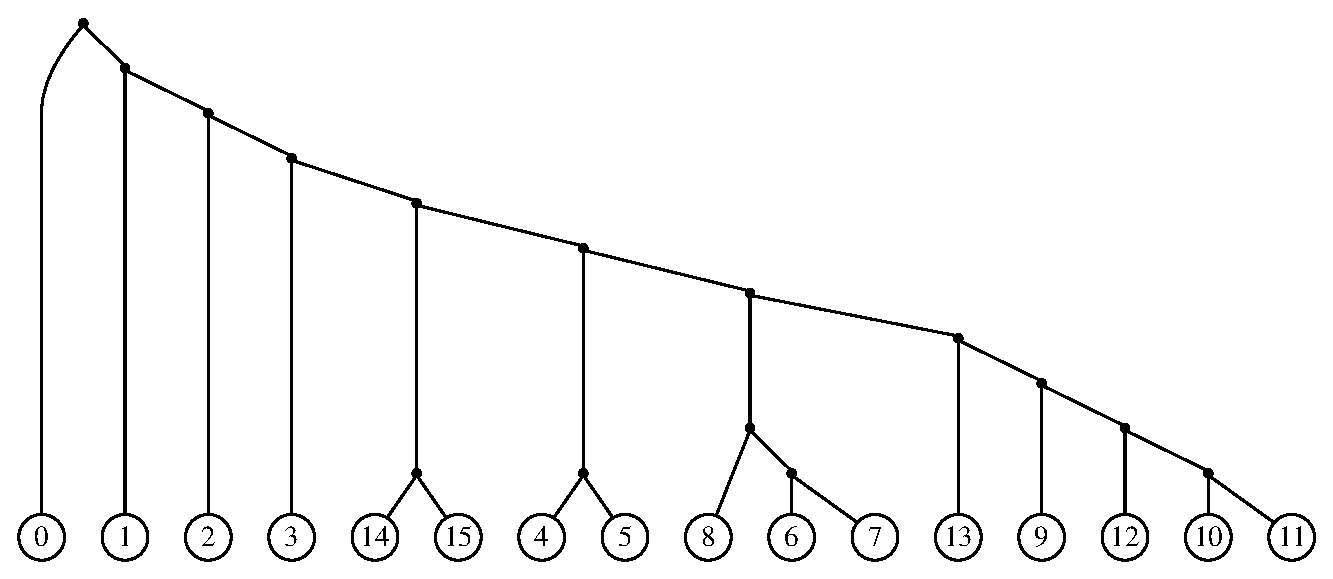
\includegraphics[width=\linewidth]{img/Grass2WaxyIts_tree0}
  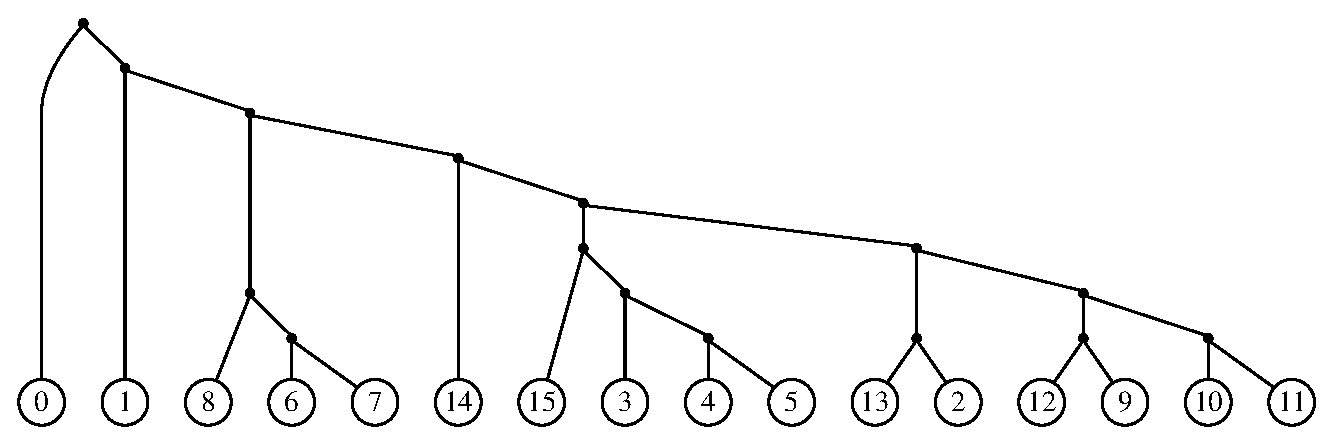
\includegraphics[width=\linewidth]{img/Grass2WaxyIts_tree1}
  \\\\\\
  \centering
  Рис. 1.1: Входные деревья для теста WaxyIts.
\end{figure}

\begin{figure}[h]
  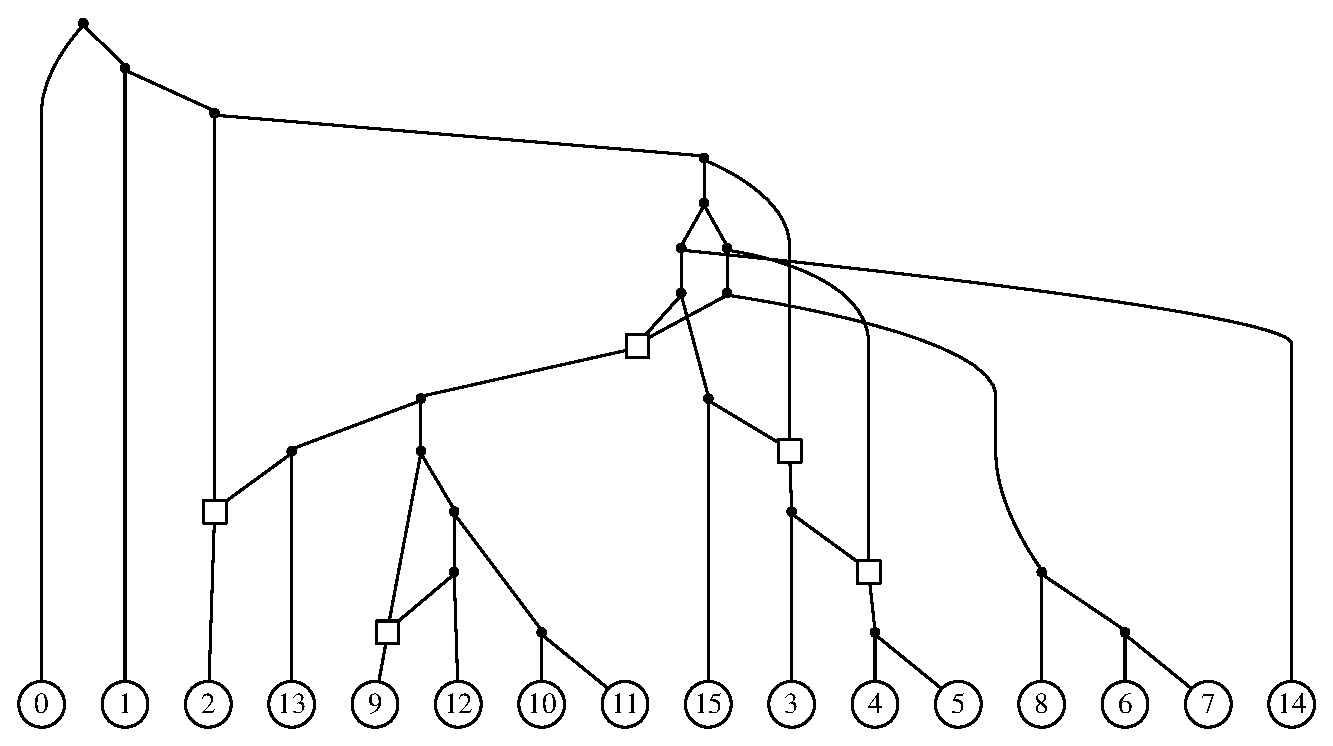
\includegraphics[width=\linewidth]{img/Grass2WaxyIts}
  \\\\\\
  \centering
  Рис. 1.2: Минимальная гибридизационная сеть для теста WaxyIts.
\end{figure}

\begin{figure}[h]
  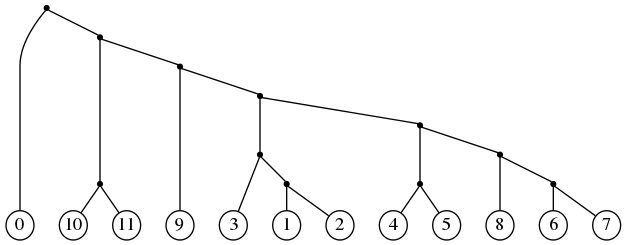
\includegraphics[width=\linewidth]{img/Grass3RbclWaxyIts_tree0}
  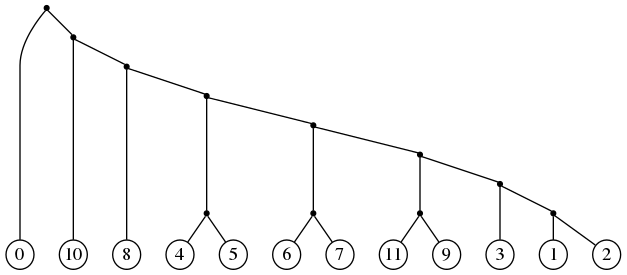
\includegraphics[width=\linewidth]{img/Grass3RbclWaxyIts_tree1}
  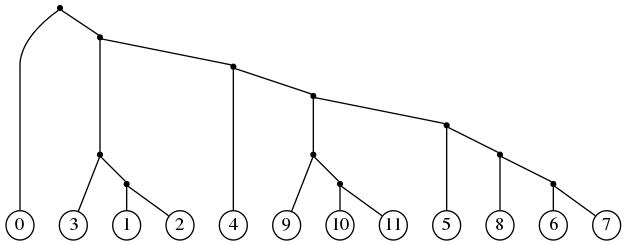
\includegraphics[width=\linewidth]{img/Grass3RbclWaxyIts_tree2}
  \\\\\\
  \centering
  Рис. 1.3: Входные деревья для теста RbclWaxyIts.
\end{figure}

\begin{figure}[h]
  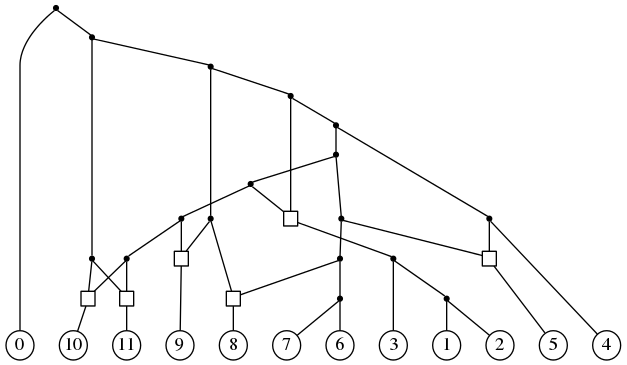
\includegraphics[width=\linewidth]{img/Grass3RbclWaxyIts}
  \\\\\\
  \centering
  Рис. 1.4: Минимальная гибридизационная сеть для теста RbclWaxyIts.
\end{figure}

\chapter{Подробные результаты тестирования} \label{AppendixB}

\begin{table}[h!]
Таблица 2.1: Подробные результаты тестирования PhyloSAT и PIRN$\mathrm{_{CH}}$. Приведены гибридизационные числа итоговых сетей. -1 означает, что не было получено никакой сети.
\\\\\\
\centering
\resizebox{0.55\textwidth}{!}{  
\begin{tabular}{l|c|c|c|c}
& PhyloSat & Время (сек) & PIRN$\mathrm{_{CH}}$ & Время (сек) \\
\hline
NdhfIts             & -1       & 1000  & -1   & 1000  \\
NdhfPhyt            & 8        & 11    & -1   & 1000  \\
NdhfRbcl            & 8        & 1     & 8    & 856   \\
NdhfRpoc            & 9        & 953   & 9    & 485   \\
NdhfWaxy            & 6        & 9     & 6    & 6     \\
PhytIts             & 8        & 45    & 8    & 373   \\
PhytRbcl            & 4        & 0     & 4    & 3     \\
PhytRpoc            & 4        & 0     & 4    & 1     \\
PhytWaxy            & 3        & 0     & 3    & 0     \\
RbclIts             & -1       & 1000  & -1   & 1000  \\
RbclRpoc            & 7        & 1000  & 7    & 43    \\
RbclWaxy            & 4        & 4     & 4    & 0     \\
RpocIts             & -1       & 1000  & -1   & 1000  \\
RpocWaxy            & 2        & 0     & 2    & 0     \\
WaxyIts             & 5        & 8     & 5    & 2     \\
NdhfPhytIts         & 13       & 1000  & -1   & 1000  \\
NdhfPhytRbcl        & 9        & 100   & -1   & 1000  \\
NdhfPhytRpoc        & 8        & 1000  & 8    & 28    \\
NdhfPhytWaxy        & 4        & 0     & 4    & 1     \\
NdhfRbclIts         & -1       & 1000  & -1   & 1000  \\
NdhfRbclRpoc        & 12       & 1000  & -1   & 1000  \\
NdhfRbclWaxy        & 5        & 67    & 5    & 0     \\
NdhfRpocIts         & -1       & 1000  & -1   & 1000  \\
NdhfRpocWaxy        & 3        & 0     & 3    & 0     \\
NdhfWaxyIts         & 8        & 1000  & 8    & 89    \\
PhytRbclIts         & 9        & 1000  & 8    & 116   \\
PhytRbclRpoc        & 6        & 12    & 6    & 3     \\
PhytRbclWaxy        & 2        & 0     & 2    & 0     \\
PhytRpocIts         & 7        & 1000  & 7    & 58    \\
PhytWaxyIts         & 4        & 0     & 4    & 0     \\
RbclRpocIts         & -1       & 1000  & -1   & 1000  \\
RbclRpocWaxy        & 3        & 0     & 3    & 0     \\
RbclWaxyIts         & 6        & 1000  & 7    & 3     \\
RpocWaxyIts         & 4        & 2     & 4    & 0     \\
NdhfPhytRbclIts     & -1       & 1000  & -1   & 1000  \\
NdhfPhytRbclRpoc    & 9        & 1000  & 10   & 279   \\
NdhfPhytRbclWaxy    & 2        & 0     & 2    & 0     \\
NdhfPhytRpocIts     & 10       & 1000  & -1   & 1000  \\
NdhfPhytWaxyIts     & 5        & 0     & 5    & 15    \\
NdhfRbclRpocIts     & -1       & 1000  & -1   & 1000  \\
NdhfRbclRpocWaxy    & 4        & 1     & 4    & 0     \\
NdhfRbclWaxyIts     & 6        & 1000  & 7    & 35    \\
NdhfRpocWaxyIts     & 5        & 42    & 5    & 2     \\
PhytRbclRpocIts     & 9        & 1000  & 8    & 364   \\
PhytRbclWaxyIts     & 2        & 0     & 2    & 0     \\
RbclRpocWaxyIts     & 5        & 34    & 5    & 2     \\
NdhfPhytRbclRpocIts & -1       & 1000  & -1   & 1000  \\
NdhfPhytRbclWaxyIts & 3        & 0     & 3    & 0     \\
NdhfRbclRpocWaxyIts & 5        & 34    & 5    & 13    \\
\end{tabular}
}
\end{table}


\end{document}
